\chapter*{Tarefa - 1}

\section*{Enunciado}

\begin{figure}[H]
\centering
\caption{Enunciado da Tarefa 1.}
\centering
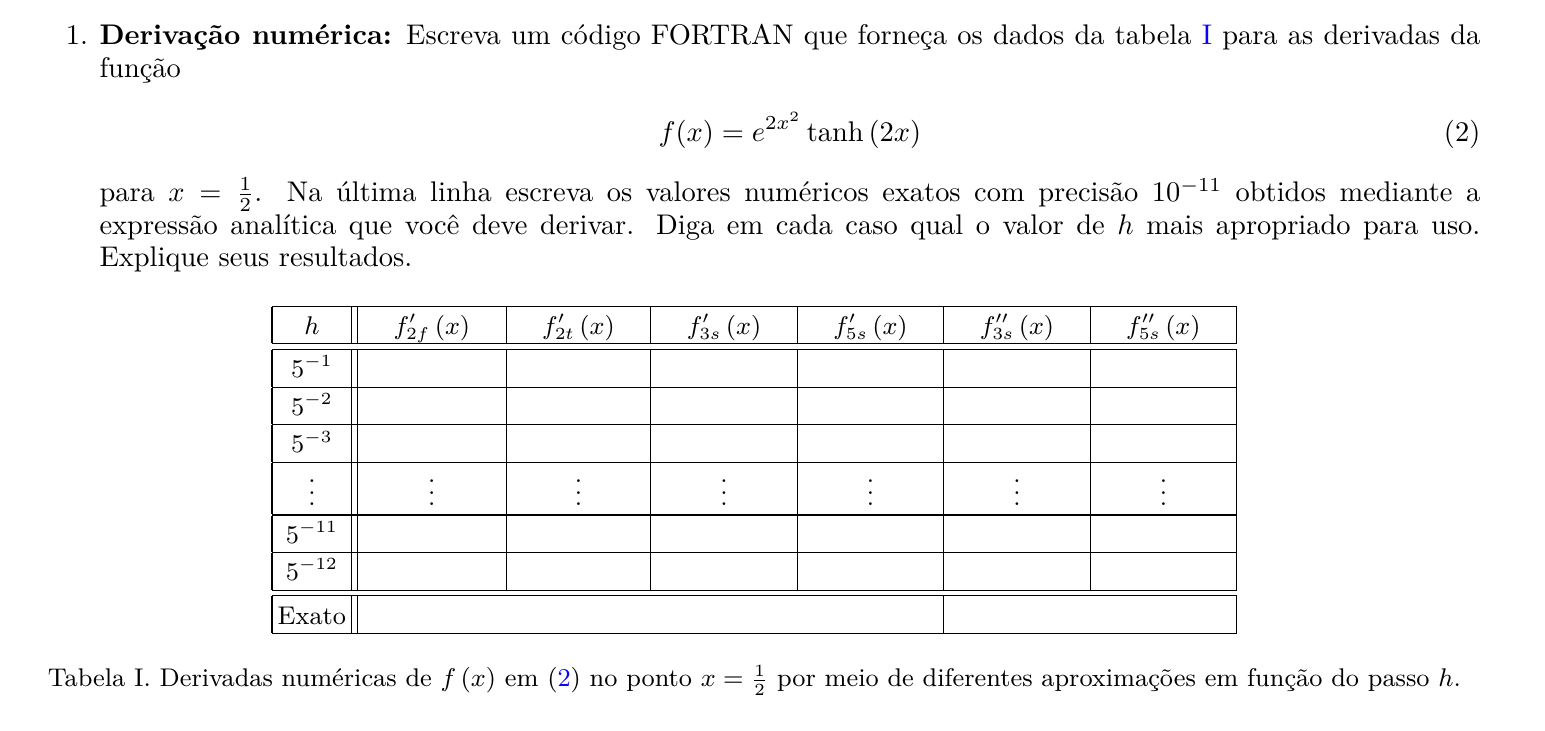
\includegraphics[width=16cm]{images/tarefa-1/enunciado-tarefa-1.png}
\caption*{Fonte: Compilado pelo Autor.}
\label{fig:tarefa 1 - Enunciado}
\end{figure}

\section*{Código}


\vspace*{1\baselineskip}

\begin{figure}[H]
\centering
\caption{Função principal do código.}
\centering

\begin{lstlisting}
        program main
        implicit real*8 (a-h,o-z)

        open(unit=1,file='saida-1-12694394.txt')
        write(1,3)

        x = 0.5d0
        do i = 1,12
            h = 5d0**(-i)
        write(1,7) i,f1(x,h),f2(x,h),f3(x,h),f4(x,h),f5(x,h),f6(x,h)
        end do
        write(1,3)

7       format('|',I3,6('|',F14.12),'|')
3       format(95('-'))
        close(1)
        end program main
\end{lstlisting}

\caption*{Fonte: Compilado pelo Autor.}
\label{fig:tarefa 1 - função principal do código}
\end{figure}

\vspace*{1\baselineskip}

\begin{figure}[H]
\centering
\caption{Função estudada.}
\centering

\begin{lstlisting}
        function f(x)
        real*8 f,x
        
        f = exp(2d0*x*x)*tanh(2d0*x)
        return
        end function f
\end{lstlisting}

\caption*{Fonte: Compilado pelo Autor.}
\label{fig:tarefa 1 - função f}
\end{figure}



\vspace*{1\baselineskip}

\begin{figure}[H]
\centering
\caption{Derivadas númericas.}
\centering

\begin{lstlisting}

        function f1(x,h)
        implicit real*8 (a-h,o-z)
        
        f1 = (f(x+h)-f(x))/h

        return
        end function f1

        function f2(x,h)
        real*8 f2,f,x,h

        f2 = (f(x)-f(x-h))/h

        return
        end function f2

        function f3(x,h)
        implicit real*8 (a-h,o-z)

        f3 = (f(x + h) - f(x - h))/(2d0*h)

        return
        end function f3

        function f4(x,h)
        implicit real*8 (a-h,o-z)

        f4 = (f(x-2d0*h)-8d0*f(x-h)+8d0*f(x+h)-f(x+2d0*h))/(12d0*h)
        return
        end function f4

        function f5(x,h)
        implicit real*8 (a-h,o-z)

        f5 = (f(x+h) -2*f(x) + f(x-h))/(h*h)

        return
        end function f5

        function f6(x,h)
        implicit real*8 (a-h,o-z)

        f6 =-f(x-2*h)+16*f(x-h)-30*f(x)+16*f(x+h)-f(x+2*h)
        f6=f6/(12*h*h)
        return
        end function f6
\end{lstlisting}

\caption*{Fonte: Compilado pelo Autor.}
\label{fig:tarefa 1 - Derivadas}
\end{figure}

\begin{figure}[H]
\centering
\caption{Segundas derivadas númericas.}
\centering

\begin{lstlisting}
        function f5(x,h)
        implicit real*8 (a-h,o-z)

        f5 = (f(x+h) -2*f(x) + f(x-h))/(h*h)

        return
        end function f5

        function f6(x,h)
        implicit real*8 (a-h,o-z)

        f6 =-f(x-2*h)+16*f(x-h)-30*f(x)+16*f(x+h)-f(x+2*h)
        f6=f6/(12*h*h)
        return
        end function f6
\end{lstlisting}

\caption*{Fonte: Compilado pelo Autor.}
\label{fig:tarefa 1 - Segundas derivadas}
\end{figure}


\newpage
\section*{Descrição do código}
O programa \texttt{main} tem como objetivo calcular numericamente 
derivadas de primeira e segunda ordem da função

\begin{equation}
	f(x) = e^{2x^2} \tanh(2x),
\end{equation}

\noindent 
utilizando diferentes fórmulas de derivadas númericas.  
Essas aproximações são avaliadas para um ponto fixo $x = 0.5$, 
variando o passo $h$ em potências decrescentes de 5, isto é:

\begin{equation}
	h = 5^{-i}, \quad i = 1, 2, \ldots, 12.
\end{equation}

\noindent
Os resultados são escritos em um arquivo de saída denominado 
\texttt{saida-1-12694394.txt}. Ademais no início do código, é 
utilizada o comando:

\vspace*{1\baselineskip}
\begin{lstlisting}
implicit real*8 (a-h,o-z)
\end{lstlisting}

\noindent
que define todas as variáveis cujos nomes começam com as letras 
de \textbf{a} a \textbf{h} e \textbf{o} a \textbf{z}  como números reais de dupla precisão.
Em seguida, o programa abre o arquivo de saída com o comando:

\vspace*{1\baselineskip}
\begin{lstlisting}
open(unit=1,file='saida-1-12694394.txt')
\end{lstlisting}

\noindent
e escreve uma linha de separação utilizando o formato definido 
pelo rótulo \texttt{3}, que imprime 95 hifens 
(\texttt{format(95('-'))}).

No bloco principal, é fixado o valor $x = 0.5$.  
O programa então entra em um laço de 12 iterações 
(\texttt{do i = 1,12}), no qual o passo $h$ é definido conforme 
a Equação (2). Para cada valor de $h$, o programa calcula seis aproximações 
numéricas das derivadas da função $f(x)$ por meio das funções 
\texttt{f1} a \texttt{f6}, gravando os resultados no arquivo de 
saída com a instrução:

\vspace*{1\baselineskip}
\begin{lstlisting}
write(1,7) i,f1(x,h),f2(x,h),f3(x,h),f4(x,h),f5(x,h),f6(x,h)
\end{lstlisting}

O formato identificado pelo rótulo \texttt{7}:

\vspace*{1\baselineskip}
\begin{lstlisting}
7   format('|',I3,6('|',F16.12),'|')
\end{lstlisting}

\noindent
organiza os resultados em colunas, contendo o número da iteração 
seguido das seis aproximações, todas com 12 casas decimais.  
Após o laço, o programa imprime novamente a linha de separação 
e fecha o arquivo com o comando:

\vspace*{1\baselineskip}
\begin{lstlisting}
close(1)
\end{lstlisting}

\subsection*{Funções auxiliares}

As funções \texttt{f1} a \texttt{f6} implementam diferentes fórmulas 
de diferenças finitas para a primeira e segunda derivadas de $f(x)$.

\begin{enumerate}
	\item \textbf{Função \texttt{f(x)}} \\
	Define a função principal:
	\begin{equation}
		f(x) = e^{2x^2} \tanh(2x).
	\end{equation}

	\item \textbf{Função \texttt{f1(x,h)}} — Derivada para frente de 2 pontos 
	(1ª derivada)
	\begin{equation}
		f'_1(x) \approx \frac{f(x+h) - f(x)}{h}.
	\end{equation}
	Essa é a aproximação de primeira ordem para a derivada.

	\item \textbf{Função \texttt{f2(x,h)}} — Derivada para trás de 2 pontos
	(1ª derivada)
	\begin{equation}
		f'_2(x) \approx \frac{f(x) - f(x-h)}{h}.
	\end{equation}
	Também é de primeira ordem, mas utiliza pontos à esquerda de $x$.

	\item \textbf{Função \texttt{f3(x,h)}} — Derivada simétrica de 3 pontos
	(1ª derivada)
	\begin{equation}
		f'_3(x) \approx \frac{f(x+h) - f(x-h)}{2h}.
	\end{equation}
	É uma aproximação de segunda ordem, mais precisa que as anteriores.

	\item \textbf{Função \texttt{f4(x,h)}} — Derivada simétrica de 5 pontos 
	de quarta ordem (1ª derivada)
	\begin{equation}
		f'_4(x) \approx 
		\frac{-f(x+2h) + 8f(x+h) - 8f(x-h) + f(x-2h)}{12h}.
	\end{equation}
	Fornece uma aproximação de quarta ordem, mais precisa para 
	a derivada primeira.

	\item \textbf{Função \texttt{f5(x,h)}} — Derivada segunda simétrica de três pontos
	(2ª derivada)
	\begin{equation}
		f''_5(x) \approx 
		\frac{f(x+h) - 2f(x) + f(x-h)}{h^2}.
	\end{equation}
	Essa é uma aproximação de segunda ordem para a derivada segunda.

	\item \textbf{Função \texttt{f6(x,h)}} — Derivada segunda simétrica de 5 pontos
	de quarta ordem (2ª derivada)
	\begin{equation}
		f''_6(x) \approx 
		\frac{-f(x+2h) + 16f(x+h) - 30f(x) 
		+ 16f(x-h) - f(x-2h)}{12h^2}.
	\end{equation}
	Essa é uma aproximação de quarta ordem, ainda mais precisa.
\end{enumerate}

\section*{Resultados}


\begin{table}[h!]
\centering
\caption{Valores de $f'(x)$ obtidos por diferentes métodos numéricos.}
\label{table:derivada-primeira}
\begin{NiceTabular}{c|cccc}[hvlines, columns-width=2.6cm]
\CodeBefore
    \rowcolor{cyan}{1}
    \rowcolors{2}{cyan!25}{cyan!15}
\Body
    \RowStyle[color=white, bold]{}
    $h = 5^{-i}$ & $f'_{2f}(x)$ & $f'_{2t}(x)$ & $f'_{3s}(x)$ & $f'_{5s}(x)$ \\ 
    5$^{-1}$  & 5.51662120 & 3.06345709 & 4.29003915 & 3.81049648 \\
    5$^{-2}$  & 4.13920591 & 3.68318855 & 3.91119723 & 3.89603900 \\
    5$^{-3}$  & 3.94222385 & 3.85128585 & 3.89675485 & 3.89615405 \\
    5$^{-4}$  & 3.90527099 & 3.88708551 & 3.89617825 & 3.89615423 \\
    5$^{-5}$  & 3.89797373 & 3.89433665 & 3.89615519 & 3.89615423 \\
    5$^{-6}$  & 3.89651798 & 3.89579056 & 3.89615427 & 3.89615423 \\
    5$^{-7}$  & 3.89622697 & 3.89608149 & 3.89615423 & 3.89615423 \\
    5$^{-8}$  & 3.89616878 & 3.89613968 & 3.89615423 & 3.89615423 \\
    5$^{-9}$  & 3.89615714 & 3.89615132 & 3.89615423 & 3.89615423 \\
    5$^{-10}$ & 3.89615481 & 3.89615365 & 3.89615423 & 3.89615423 \\
    5$^{-11}$ & 3.89615435 & 3.89615411 & 3.89615423 & 3.89615424 \\
    5$^{-12}$ & 3.89615418 & 3.89615423 & 3.89615421 & 3.89615421 \\
    \hline
    \textbf{Exato} & \multicolumn{4}{c}{3.89615422946} \\
\end{NiceTabular}

\caption*{Fonte: Compilado pelo Autor}
\end{table}

\begin{table}[h!]
\centering
\caption{Valores de $f''(x)$ obtidos por diferentes métodos numéricos.}
\label{table:derivada-segunda}
\begin{NiceTabular}{c|cc}[hvlines, columns-width=2.6cm]
\CodeBefore
    \rowcolor{cyan}{1}
    \rowcolors{2}{cyan!25}{cyan!15}
\Body
    \RowStyle[color=white, bold]{}
    $h = 5^{-i}$ & $f''_{3s}(x)$ & $f''_{5s}(x)$ \\ 
    5$^{-1}$  & 12.26582057 & 11.19954015 \\
    5$^{-2}$  & 11.40043402 & 11.36563532 \\
    5$^{-3}$  & 11.36724925 & 11.36586850 \\
    5$^{-4}$  & 11.36592409 & 11.36586887 \\
    5$^{-5}$  & 11.36587108 & 11.36586887 \\
    5$^{-6}$  & 11.36586891 & 11.36586877 \\
    5$^{-7}$  & 11.36587027 & 11.36586936 \\
    5$^{-8}$  & 11.36582690 & 11.36579019 \\
    5$^{-9}$  & 11.36379402 & 11.36301757 \\
    5$^{-10}$ & 11.39259314 & 11.40141640 \\
    5$^{-11}$ & 11.64670302 & 11.42612153 \\
    5$^{-12}$ & -13.23488980 & -23.16105715 \\
    \hline
    \textbf{Exato} & \multicolumn{2}{c}{11.36586887467} \\
\end{NiceTabular}

\caption*{Fonte: Compilado pelo Autor}
\end{table}


\begin{landscape}
\begin{table}[H]
\centering
\caption{Valores de $f'(x)$ e $f''(x)$ obtidos por diferentes métodos numéricos.}
\label{table:derivadas}
\begin{NiceTabular}{c|cccccc}[hvlines, columns-width=2.6cm]
\CodeBefore
    \rowcolor{cyan}{1}
    \rowcolors{2}{cyan!25}{cyan!15}
\Body
    \RowStyle[color=white, bold]{}
    $h = 5^{-i}$ & $f'_{2f}(x)$ & $f'_{2t}(x)$ & $f'_{3s}(x)$ & $f'_{5s}(x)$ & $f''_{3s}(x)$ & $f''_{5s}(x)$ \\ 
    5$^{-1}$  & 5.51662120 & 3.06345709 & 4.29003915 & 3.81049648 & 12.26582057 & 11.19954015 \\
    5$^{-2}$  & 4.13920591 & 3.68318855 & 3.91119723 & 3.89603900 & 11.40043402 & 11.36563532 \\
    5$^{-3}$  & 3.94222385 & 3.85128585 & 3.89675485 & 3.89615405 & 11.36724925 & 11.36586850 \\
    5$^{-4}$  & 3.90527099 & 3.88708551 & 3.89617825 & 3.89615423 & 11.36592409 & 11.36586887 \\
    5$^{-5}$  & 3.89797373 & 3.89433665 & 3.89615519 & 3.89615423 & 11.36587108 & 11.36586887 \\
    5$^{-6}$  & 3.89651798 & 3.89579056 & 3.89615427 & 3.89615423 & 11.36586891 & 11.36586877 \\
    5$^{-7}$  & 3.89622697 & 3.89608149 & 3.89615423 & 3.89615423 & 11.36587027 & 11.36586936 \\
    5$^{-8}$  & 3.89616878 & 3.89613968 & 3.89615423 & 3.89615423 & 11.36582690 & 11.36579019 \\
    5$^{-9}$  & 3.89615714 & 3.89615132 & 3.89615423 & 3.89615423 & 11.36379402 & 11.36301757 \\
    5$^{-10}$ & 3.89615481 & 3.89615365 & 3.89615423 & 3.89615423 & 11.39259314 & 11.40141640 \\
    5$^{-11}$ & 3.89615435 & 3.89615411 & 3.89615423 & 3.89615424 & 11.64670302 & 11.42612153 \\
    5$^{-12}$ & 3.89615418 & 3.89615423 & 3.89615421 & 3.89615421 & -13.23488980 & -23.16105715 \\
    \hline
    \textbf{Exato} 
    & \multicolumn{4}{c|}{3.89615422946} 
    & \multicolumn{2}{c}{11.36586887467} \\
\end{NiceTabular}
\caption*{Fonte: Compilado pelo Autor}
\end{table}
\end{landscape}


\begin{figure}[h!]
\centering
\caption{Dados salvos no arquivo de saida para a Tarefa - 1.}
\centering
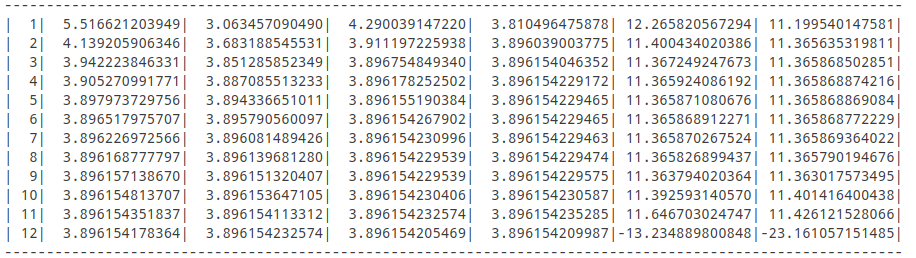
\includegraphics[width=16cm]{images/tarefa-1/tabela-1-tarefa-1.png}
\caption*{Fonte: Compilado pelo Autor.}
\label{fig:tarefa 1 - Tabela 1}
\end{figure}


\begin{figure}[H]
\centering
\caption{Gráfico das funções estudadas.}
\centering
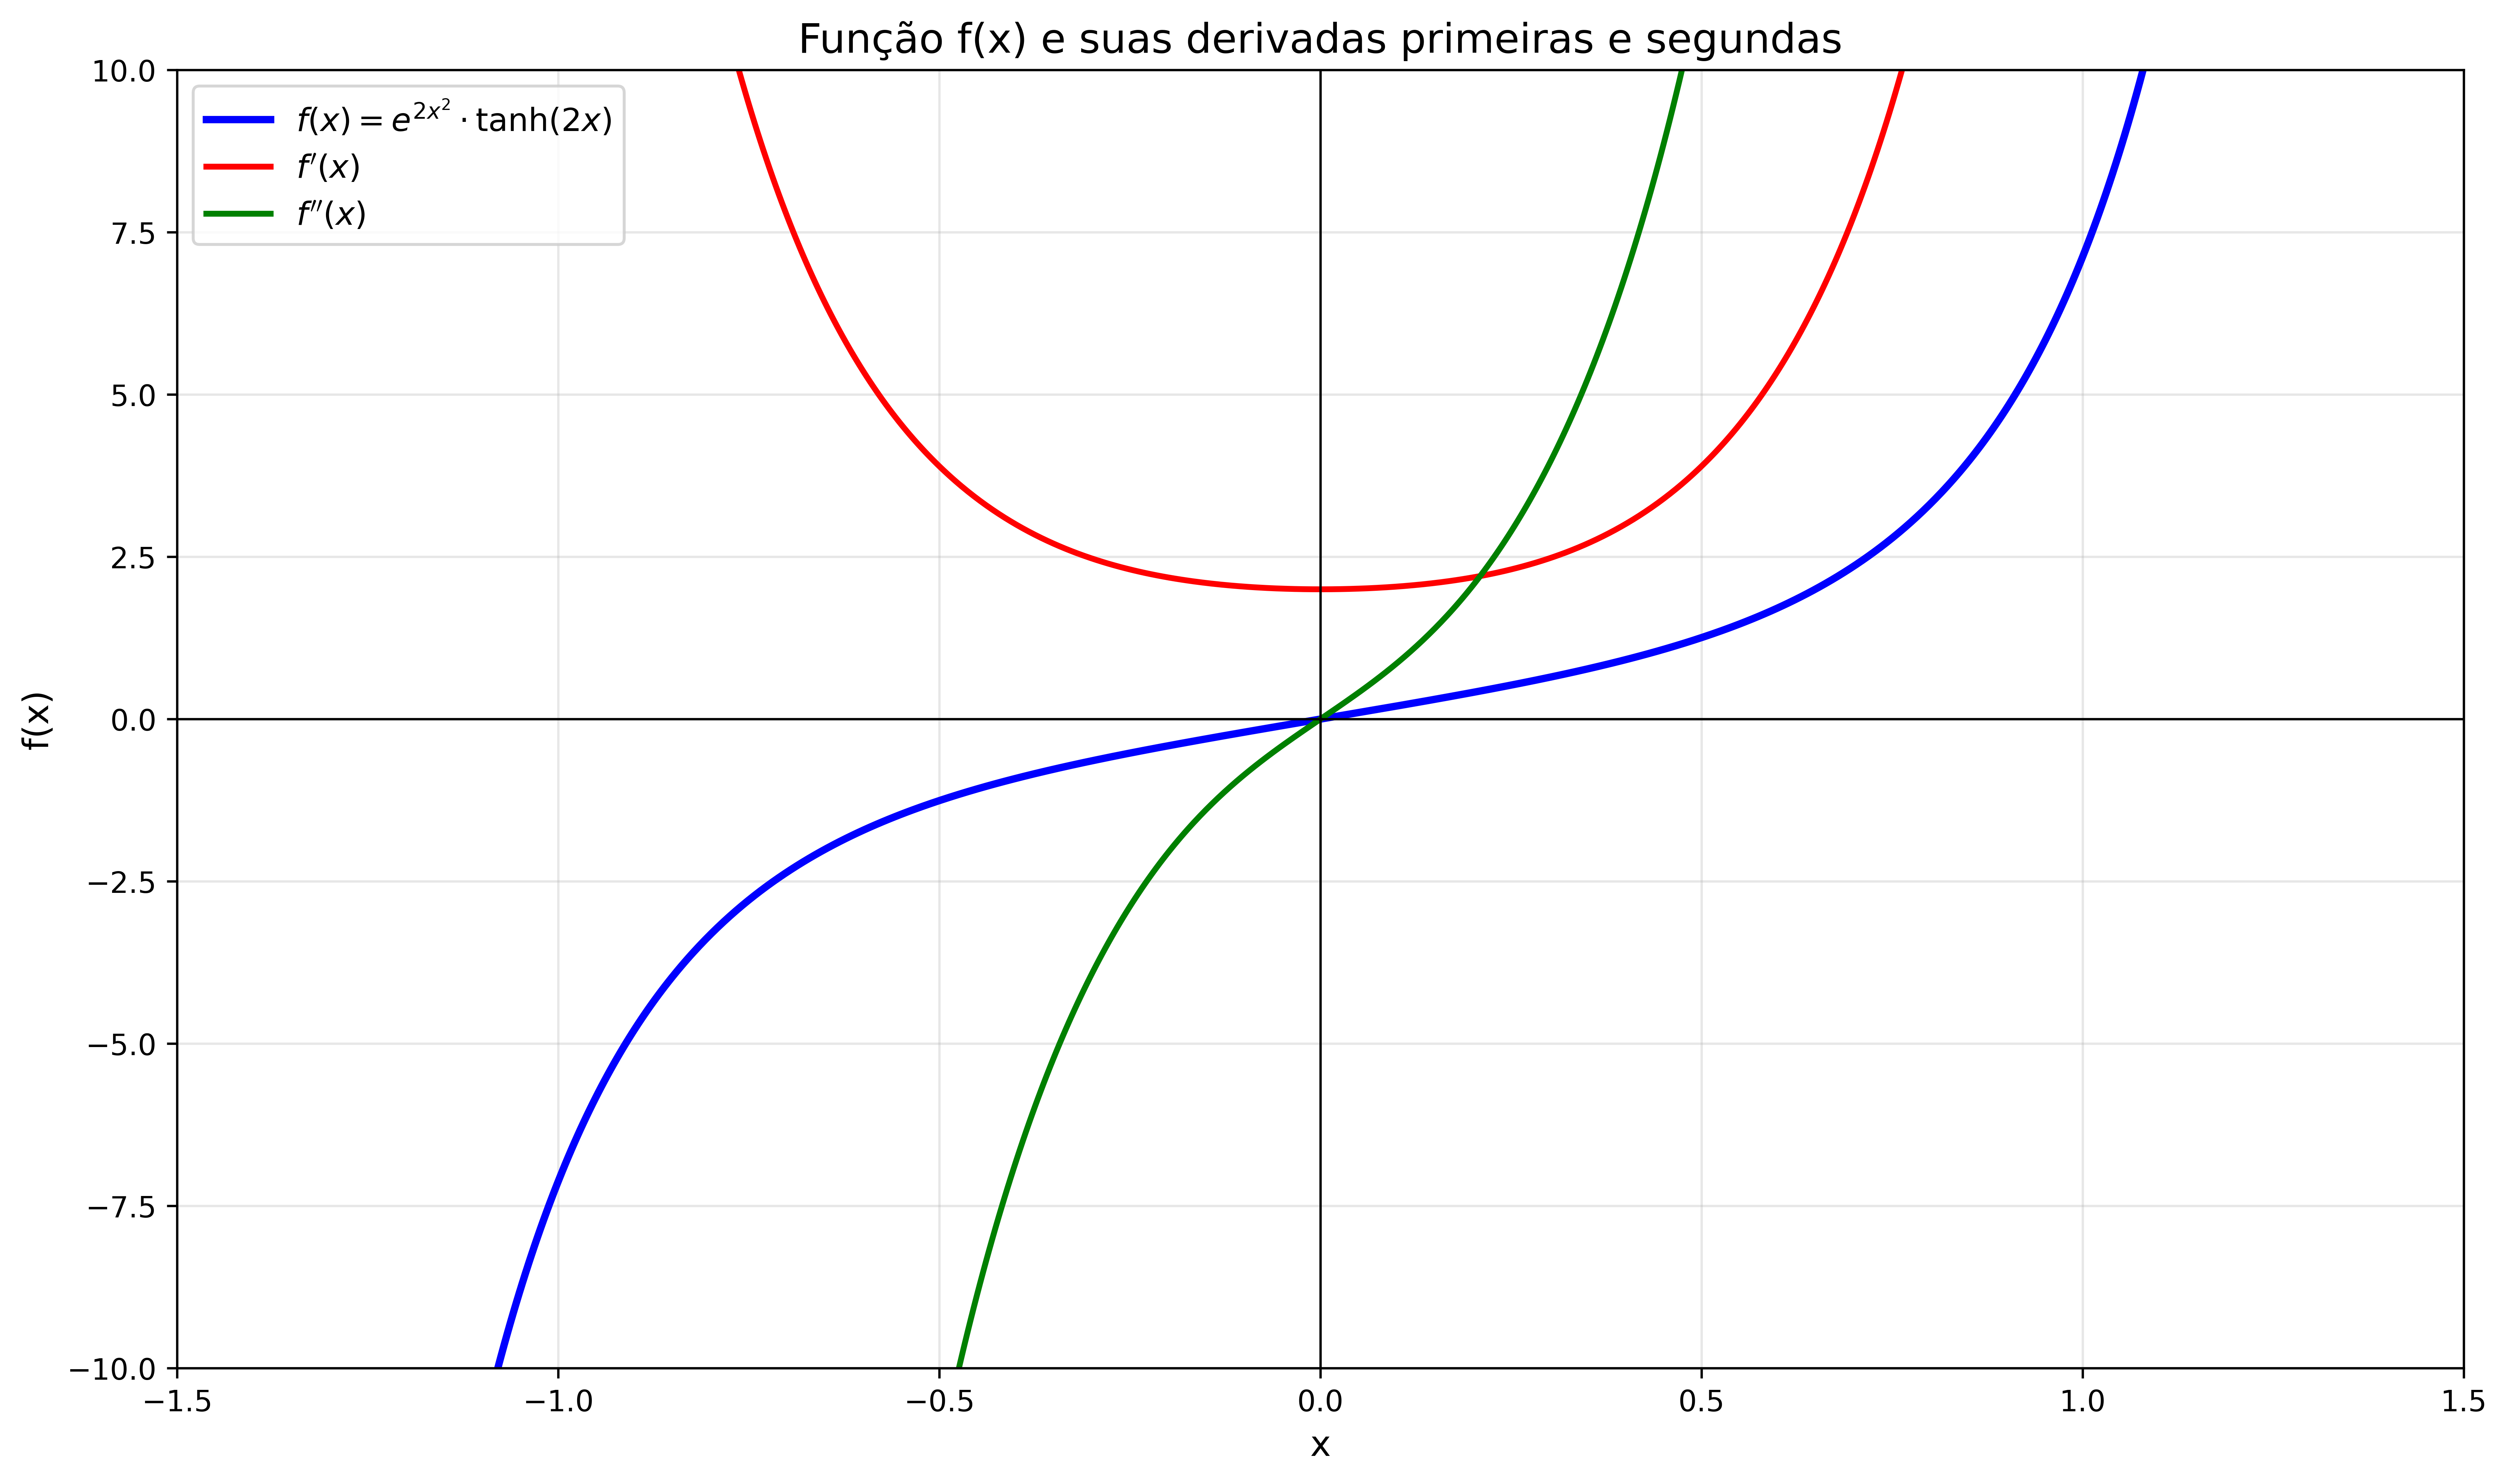
\includegraphics[width=16cm]{images/tarefa-1/tarefa-1-graf-1.png}
\caption*{Fonte: Compilado pelo Autor.}
\label{fig:tarefa 1 - Gráfico 1}
\end{figure}

\begin{figure}[H]
\centering
\caption{Gráfico das funções estudadas marcando o ponto $x=0.50$.}
\centering
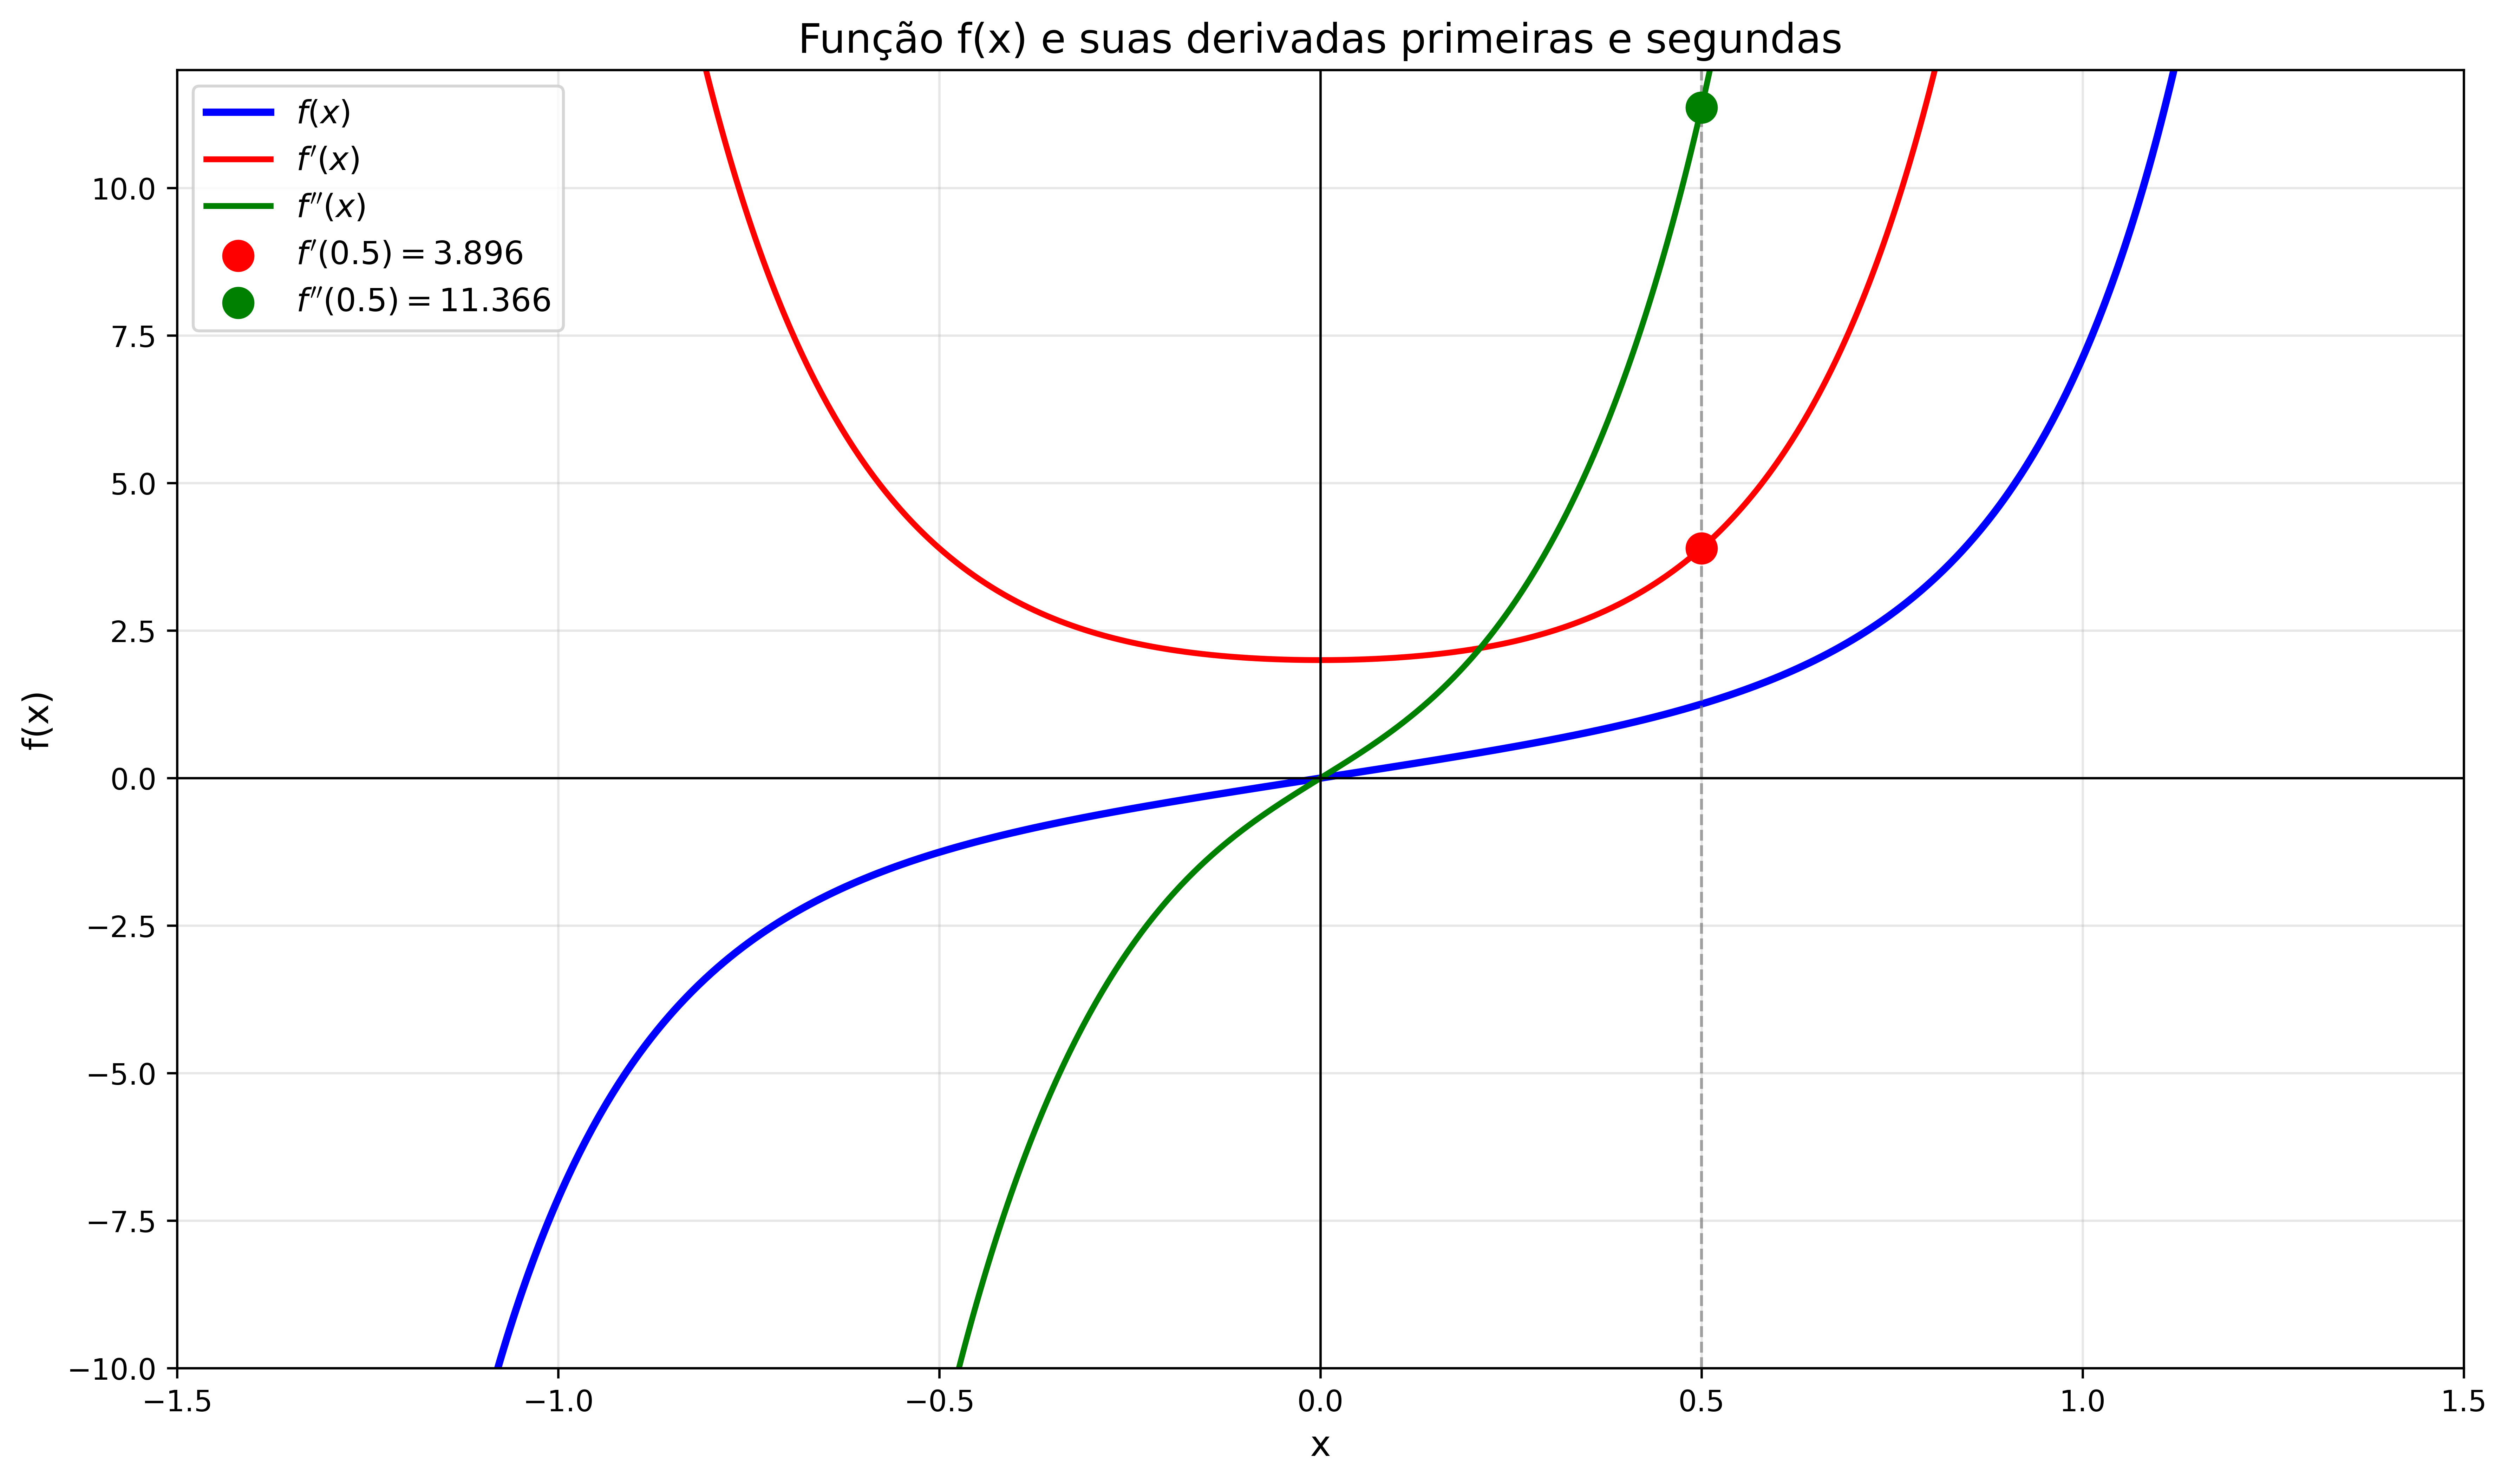
\includegraphics[width=16cm]{images/tarefa-1/tarefa-1-graf-2.png}
\caption*{Fonte: Compilado pelo Autor.}
\label{fig:tarefa 1 - Gráfico 2}
\end{figure}

